\subsection{Ola Language Compiler Frontend}

\subsubsection{Introduction}
This section introduces the key components and functionalities of the Ola language compiler frontend. We will discuss the process of lexical analysis, syntax parsing, Abstract Syntax Tree (AST) generation, semantic analysis, and LLVM Intermediate Representation (IR) generation in detail.

The processing flow of the compiler front-end is shown in the following diagram \ref{fig:ola-lang-compiler-frontend}:

\begin{figure}[!ht]
    \centering
    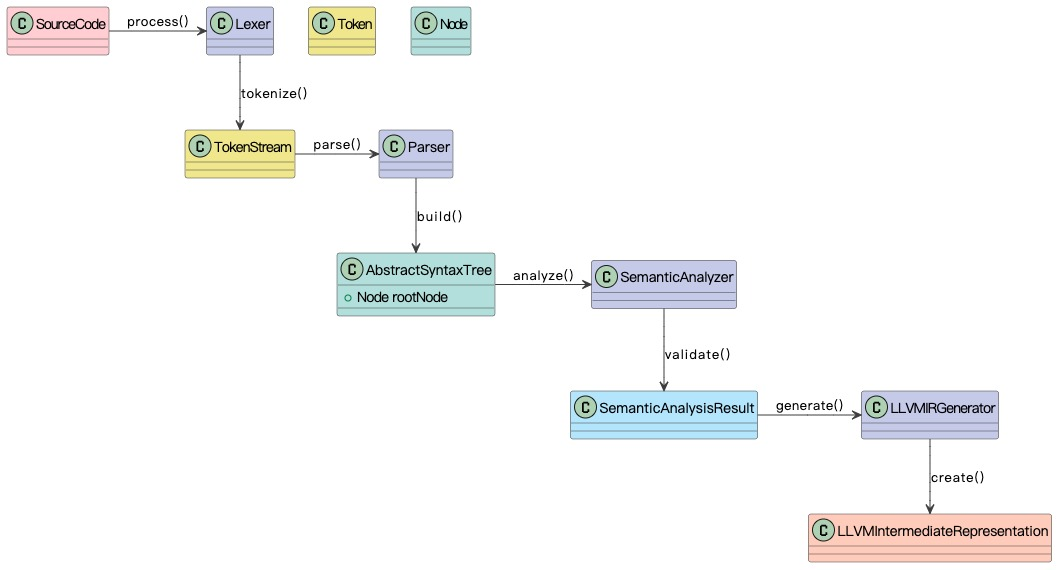
\includegraphics[width=0.8\textwidth]{ola-lang-compiler-frontend.jpg}
    \caption{Ola-lang Compiler Frontend}
    \label{fig:ola-lang-compiler-frontend}
\end{figure}

\subsubsection{Lexical Analysis}
Lexical analysis is the first stage of the compiler frontend. In this phase, the goal is to break down the source code into a series of tokens. The Ola language lexer will handle the following elements:
\begin{itemize}
\item Keywords
\item Identifiers
\item Operators
\item Literals (such as strings, numbers, and boolean values)
\item Comments
\item Delimiters (such as parentheses and commas)
\end{itemize}
Additionally, the lexer will eliminate whitespace and comments, ensuring a clean token stream for the next stage.

\subsubsection{Syntax Parsing}
Syntax parsing is the process of transforming the tokens generated in the lexical analysis phase into an Abstract Syntax Tree (AST). The Ola language compiler will implement a top-down parser, such as a Recursive Descent Parser, to support Ola language's grammar.

This section will also discuss the implementation of error handling and recovery mechanisms, ensuring that the parser can handle syntax errors gracefully and provide helpful error messages to the user.

\subsubsection{Abstract Syntax Tree (AST) Generation}
During the syntax parsing phase, the parser will generate an AST representing the program's structure. This section will explain the design of the AST data structures and the process of constructing the AST during parsing. Additionally, it will cover the benefits of using an AST, such as enabling easier manipulation and analysis of the code's structure.

The OLA compiler seamlessly integrates the Lexical Analysis, Syntax Parsing, and Abstract Syntax Tree (AST) Generation processes, forming a cohesive and efficient pipeline. By leveraging the LALRPOP framework, these stages work in harmony, transforming the OLA source code into an AST representation that is suitable for subsequent compiler phases. This unified approach not only simplifies the implementation but also enhances the performance and robustness of the OLA compiler.

By following these steps, the compiler can efficiently convert the Ola source code text into a sequence of tokens:

\begin{itemize}

  \item 1. The first step in implementing the lexical analysis phase of the Ola compiler is to define lexer rules for various token categories, including keywords, identifiers, literals, and operators. These rules should be based on the provided EBNF grammar rules. We created a file named Ola.lalrpop that describes Ola's EBNF grammar rules.

  \item 2. After defining the lexer rules, the next step is to integrate the lexer with the parser. This can be achieved by using the \texttt{lexer} attribute in LALRPOP grammar rules. The \texttt{lexer} attribute specifies which lexer rule should be used to recognize a particular grammar production.

  \item 3. Ola compiler provides error handling and reporting. If the lexer encounters an unexpected character or a malformed token, it generates an error with the corresponding position in the input text. This information can be used to provide helpful error messages to the user.

\end{itemize}

Once the lexical analysis phase is complete, the generated sequence of tokens can be passed to the parser, which will construct an abstract syntax tree (AST) based on the defined grammar rules. This AST can then be further processed by subsequent phases of the Ola compiler, such as semantic analysis, optimization, and code generation, ultimately producing executable code for the target platform.

By leveraging the powerful LALRPOP framework, the Ola compiler can efficiently perform lexical analysis and provide robust error handling, ensuring that the compiler is user-friendly and capable of handling complex Ola source code.

\subsubsection{Semantic Analysis}

The Semantic Analysis phase of the Ola compiler is an extensive process that ensures the program's correctness and consistency. As previously mentioned, this phase consists of several sub-tasks. Here, we delve deeper into each sub-task, providing a more detailed and comprehensive explanation of the process

\textbf{Symbol Resolution}: The compiler analyzes the program's scope and context to resolve symbols accurately. It distinguishes between local and global variables, function declarations, and type definitions. The symbol table, which holds information about each symbol, is updated as the compiler traverses the AST. During this process, the compiler also checks for naming conflicts and multiple declarations, ensuring that the program adheres to Ola's scoping rules.

\textbf{LibFunction Identification}: In the semantic analysis phase, we will identify all libFunction names that users call. We will also construct prototype code for these LibFunctions and verify whether the parameters used to call them match the parameter types and number in the prototype code. If there is a match, we will record them for easy processing of IR generation for Lib Functions in subsequent LLVM IR generation phases.

\textbf{Type Checking}: The compiler ensures that each operation and expression in the program involves operands of compatible types. In this stage, the compiler also infers the types of expressions when necessary and enforces type constraints for function calls, assignments, and arithmetic operations.

\textbf{Control Flow Analysis}: In addition to checking for unreachable code and infinite loops, the control flow analysis process verifies that:

\begin{itemize}
 \item All code paths in a function that should return a value must end with a return statement.
 \item Break and continue statements appear only within loops.
 \item Variables are declared before they are used.
\end{itemize}

\textbf{Constant Expression Evaluation}: During this step, the compiler performs the following tasks:

\begin{itemize}
  \item Evaluates arithmetic and bitwise operations on constant expressions at compile-time, ensuring that the generated code is more efficient.

  \item Detects potential errors, such as undefined behavior or array index out-of-bounds, by evaluating expressions that involve constants.

  \item Folds constant expressions, such as mathematical operations or string concatenations, reducing the code size and improving execution efficiency.

\end{itemize}

\textbf{Semantic Validation}: The final step of the semantic analysis phase consists of several validation checks, including:

\begin{itemize}
  \item Verifying that variables are initialized before they are used.
  \item Ensuring that variables, functions, and types are declared only once within a given scope.
  \item Checking that all required function arguments are provided and that excess arguments are not supplied.
  \item Validating that return statements are used correctly within functions.

\end{itemize}

The Semantic Analysis phase is crucial for the robustness and correctness of the Ola compiler. By performing these comprehensive checks, the compiler can guarantee that the generated code adheres to the language's semantic rules and is free from errors that might lead to unexpected behavior during execution. With a semantically verified AST, the Ola compiler proceeds to the subsequent phases of the compilation process, ensuring the efficient translation of the source code into executable code tailored for the Ola VM.

\subsubsection{LLVM Intermediate Representation (IR) Generation}

The LLVM IR Generation phase is a crucial step in the OLA compiler, as it translates the Abstract Syntax Tree (AST) obtained from the semantic analysis into LLVM Intermediate Representation (IR). This phase leverages the Inkwell framework, a powerful and user-friendly library that simplifies the process of generating LLVM IR code in Rust.

\subsubsection*{Inkwell Initialization}

Initialize the Inkwell context by creating a new \texttt{Context} object. Set up the target information by querying the target machine properties, such as target triple, data layout, and target-specific optimization levels. This information helps in generating the correct LLVM IR code tailored for the target architecture.

The pseudocode is shown below:

\begin{lstlisting}[language=Rust]
  // Create a new LLVM context
  let context = Context::create();
  let module = context.create_module(name);
  let builder = context.create_builder();
\end{lstlisting}
\subsubsection*{Lib IR Generation}

Before generating LLVM IR for user-defined functions, the compiler will first generate LLVM IR for previously called lib functions, prophet functions, and builtin functions. These functions have fixed logic that Ola contract developers will not change.

The pseudocode is shown below:

\begin{lstlisting}[language=Rust]
  declare_builtins(bin)
  declare_prophets(bin)
  
  for each lib function in ns.called_lib_functions:
      if lib function == "u32_sqrt":
          define function u32_sqrt(value: i64) -> i64:
              root = prophet_u32_sqrt(value)
              builtin_range_check(root)
              root_squared = root * root
              builtin_assert(root_squared, value)
              return root
      else if lib function == "u32_xxx":
          // do nothing
      else:
          // do nothing
  
\end{lstlisting}
\subsubsection*{AST Traversal}

Traverse the AST using a depth-first approach. Focus on visiting function nodes, as they represent the main building blocks of the Ola program. For each function node encountered, generate its corresponding LLVM IR.

The pseudocode is shown below:

\begin{lstlisting}[language=Rust]
  fn traverse_ast(node: &AstNode) {
    if let AstNode::Function(func) = node {
        generate_function(&func);
    }

    for child in node.children() {
        traverse_ast(child);
    }
}
\end{lstlisting}

\subsubsection*{Function Generation}

For each Ola function, create a corresponding LLVM function by invoking the \texttt{add\_function} method on the Inkwell module. Map the Ola function's return type and argument types to their corresponding LLVM types using a custom type mapping function. Add the function arguments with their respective types to the LLVM function using the \texttt{append\_parameter} method.

The pseudocode is shown below:

\begin{lstlisting}[language=Rust]
  fn generate_function(func: &OlaFunction) -> LLVMFunction {
    // Map OLA function type to LLVM function type
    let func_type = map_ola_type_to_llvm_type(&func.return_type);
    let llvm_func = context.create_function(func.name, func_type);

    // Add function arguments
    for arg in &func.arguments {
        let llvm_arg_type = map_ola_type_to_llvm_type(&arg.type);
        llvm_func.add_argument(llvm_arg_type, arg.name);
    }

    // Create a builder and position it at the entry block
    let builder = context.create_builder();
    builder.position_at_end(&llvm_func.entry);

    // Process each statement in the function body
    for stmt in &func.body {
        process_statement(stmt, &builder);
    }

    // Return the generated LLVM function
    llvm_func
}
\end{lstlisting}

\subsubsection*{Statement Processing}

Based on the type of statement encountered in the function body, generate the appropriate LLVM IR instructions. For expression statements, process the expression and generate the corresponding LLVM IR code. For variable declaration statements, allocate memory for the variable on the stack using the \texttt{build\_alloca} method, and store its initial value using the \texttt{build\_store} method. For control flow constructs, such as loops and conditionals, generate appropriate branching instructions using methods like \texttt{build\_conditional\_branch} and \texttt{build\_loop}.

The pseudocode is shown below:

\begin{lstlisting}[language=Rust]
  fn process_statement(stmt: &Statement, builder: &Builder) {
    match stmt {
        Statement::Expression(expr) => process_expression(expr, builder),
        Statement::VariableDeclaration(var_decl) => process_variable_declaration(var_decl, builder),
        // ... other statement types
    }
}
\end{lstlisting}

\subsubsection*{Expression Processing}

Process each expression encountered in the function body and generate the corresponding LLVM IR instructions. This includes handling arithmetic operations, logical operations, and control flow constructs (such as if-else expressions). For each type of expression, call the appropriate function to generate the LLVM IR code. For example, for binary expressions, generate the appropriate arithmetic or logical operation using methods like \texttt{build\_add}, \texttt{build\_mul}, or \texttt{build\_and}. For function calls, generate the \texttt{call} instruction using the \texttt{build\_call} method.


The pseudocode is shown below:

\begin{lstlisting}[language=Rust]
  fn process_expression(expr: &Expression, builder: &Builder) -> LLVMValue {
    match expr {
        Expression::BinaryExpression(op, lhs, rhs) => generate_binary_expression(op, lhs, rhs, builder),
        Expression::IfExpression(cond, then_expr, else_expr) => generate_if_expression(cond, then_expr, else_expr, builder),
        // ... other expressions
    }
}
\end{lstlisting}

\subsubsection*{Type Mapping}

Type Mapping is a crucial function that needs to be implemented in order to convert Ola types into their corresponding LLVM types. This mapping function should handle all Ola types, including basic (such as u32, u64, and u256) and complex types (such as structs and arrays). It's important to note that the Ola language is based on the Field type at its core, with various integer types built upon it. The Field Order is \texttt{0xFFFFFFFF00000001}. To fully represent a field element, we create an integer type using the method \texttt{context.i64\_type()}. For complex types such as structs and arrays, custom LLVM types can be created using methods like \texttt{context.struct\_type()} and \texttt{context.array\_type()}.

The pseudocode is shown below:

\begin{lstlisting}[language=Rust]
  fn map_ola_type_to_llvm_type(ola_type: &OlaType) -> LLVMType {
    match ola_type {
        OlaType::Field => context.i64_type(),
        OlaType::U32 => context.i32_type(),
        OlaType::U64 => context.i64_type(),
        OlaType::U256 => context.array_type(context.i64_type(), 4),
        OlaType::Struct(name) => context.struct_type(&structs[name].fields, false),
        OlaType::Array(elem_type, size) => context.array_type(map_ola_type_to_llvm_type(elem_type), *size),
        // ... other types
    }
}
\end{lstlisting}